\documentclass[conference]{IEEEtran}
\usepackage{fontspec}
\setmainfont{texgyretermes}[Extension=.otf, UprightFont=*-regular, BoldFont=*-bold, ItalicFont=*-italic, BoldItalicFont=*-bolditalic]
\usepackage{graphicx}
\usepackage{booktabs}
\usepackage{array}
\usepackage{xcolor}
\usepackage{listings}
\usepackage{tikz}
\usetikzlibrary{positioning,arrows.meta}
\usepackage[hidelinks]{hyperref}

% Results that are not measured yet. Search for PENDING before submitting.
\newcommand{\pending}[1]{\textcolor{red}{\textbf{[PENDING: #1]}}}
\newcommand{\code}[1]{\texttt{\detokenize{#1}}}

\lstset{basicstyle=\ttfamily\scriptsize, columns=fullflexible, breaklines=true,
  frame=single, framerule=0.3pt, aboveskip=4pt, belowskip=4pt}

\begin{document}

\title{Hardening a Private Network Service Platform:\\
Resilience, Isolation and Fault Diagnosis on Four macOS Hosts}

\author{\IEEEauthorblockN{Team 1: Harshita, Yashi, Manan, Akhil}
\IEEEauthorblockA{Computer Networks Course Project, Phase 2 Report\\
Repository: \url{https://github.com/AkhilMishra2216/CN_Team1}}}

\maketitle

\begin{abstract}
In Phase 1 we built a private service on four macOS laptops: a dnsmasq
resolver answers for \code{app.team1.test}, an nginx edge terminates TLS
and load-balances HTTP requests across two Python backends, and packet
captures show every layer of a single request. Phase 2 hardens the same
network without rebuilding it. We add a backup DNS resolver, use a 30\,s
TTL to observe caching during a record change, restrict the backend ports
to the edges with the macOS packet filter, demonstrate passive health
checks in nginx, and move traffic to a standby edge with a DNS cutover.
Each change is tested by deliberately breaking a component and recording
what the client sees. Measured so far: the backup resolver answers
the project names from a second host, the firewall refuses direct backend
access while traffic through the edge continues, and nginx moves requests
to the surviving backend when one stops. \pending{failover, TTL expiry and
edge cutover results}.
\end{abstract}

\begin{IEEEkeywords}
DNS failover, TTL, reverse proxy, load balancing, TLS, packet filter,
high availability, troubleshooting
\end{IEEEkeywords}

\section{Introduction}
The project asks how a request for a private name travels from a client
to a server and back, and how that path behaves when parts of it fail.
Phase 1 (\emph{Build \& Observe}) answered the first question with a
working system and packet evidence. Phase 2 (\emph{Harden \& Recover})
answers the second: which failures the system now survives, which it
does not, and how a fault is located layer by layer. The application is
deliberately trivial; every mechanism studied here is a network
mechanism.

Section~\ref{sec:p1} summarises the Phase 1 system. Section~\ref{sec:design}
describes the Phase 2 extensions, Section~\ref{sec:results} the tests and
results, Section~\ref{sec:trouble} the problems we diagnosed, and
Section~\ref{sec:discussion} what remains a single point of failure.

\section{Phase 1 System (Summary)}\label{sec:p1}

\subsection{Topology and roles}
All four Macs share one Wi-Fi LAN, 10.7.0.0/19 with gateway 10.7.0.1.
Table~\ref{tab:roles} lists the roles and the addresses used in Phase 2.
The lab DHCP server reassigned every address between the phases; the
Phase 1 evidence keeps the addresses it was recorded with.

\begin{table}[t]
\caption{Machines, Addresses and Roles}\label{tab:roles}
\centering\footnotesize
\begin{tabular}{@{}l l p{4.6cm}@{}}
\toprule
Host & IPv4 & Role (Phase 2 additions in italics)\\
\midrule
Mac 1 & 10.7.18.129 & Primary DNS (dnsmasq), client; \emph{TTL/cutover client}\\
Mac 2 & 10.7.31.128 & Edge: nginx reverse proxy, TLS, load balancer\\
Mac 3 & 10.7.10.192 & Backend A :3001; \emph{backup DNS, standby edge, firewall}\\
Mac 4 & 10.7.12.3 & Backend B :3002, main client; \emph{firewall}\\
\bottomrule
\end{tabular}
\end{table}

\begin{figure}[t]
\centering
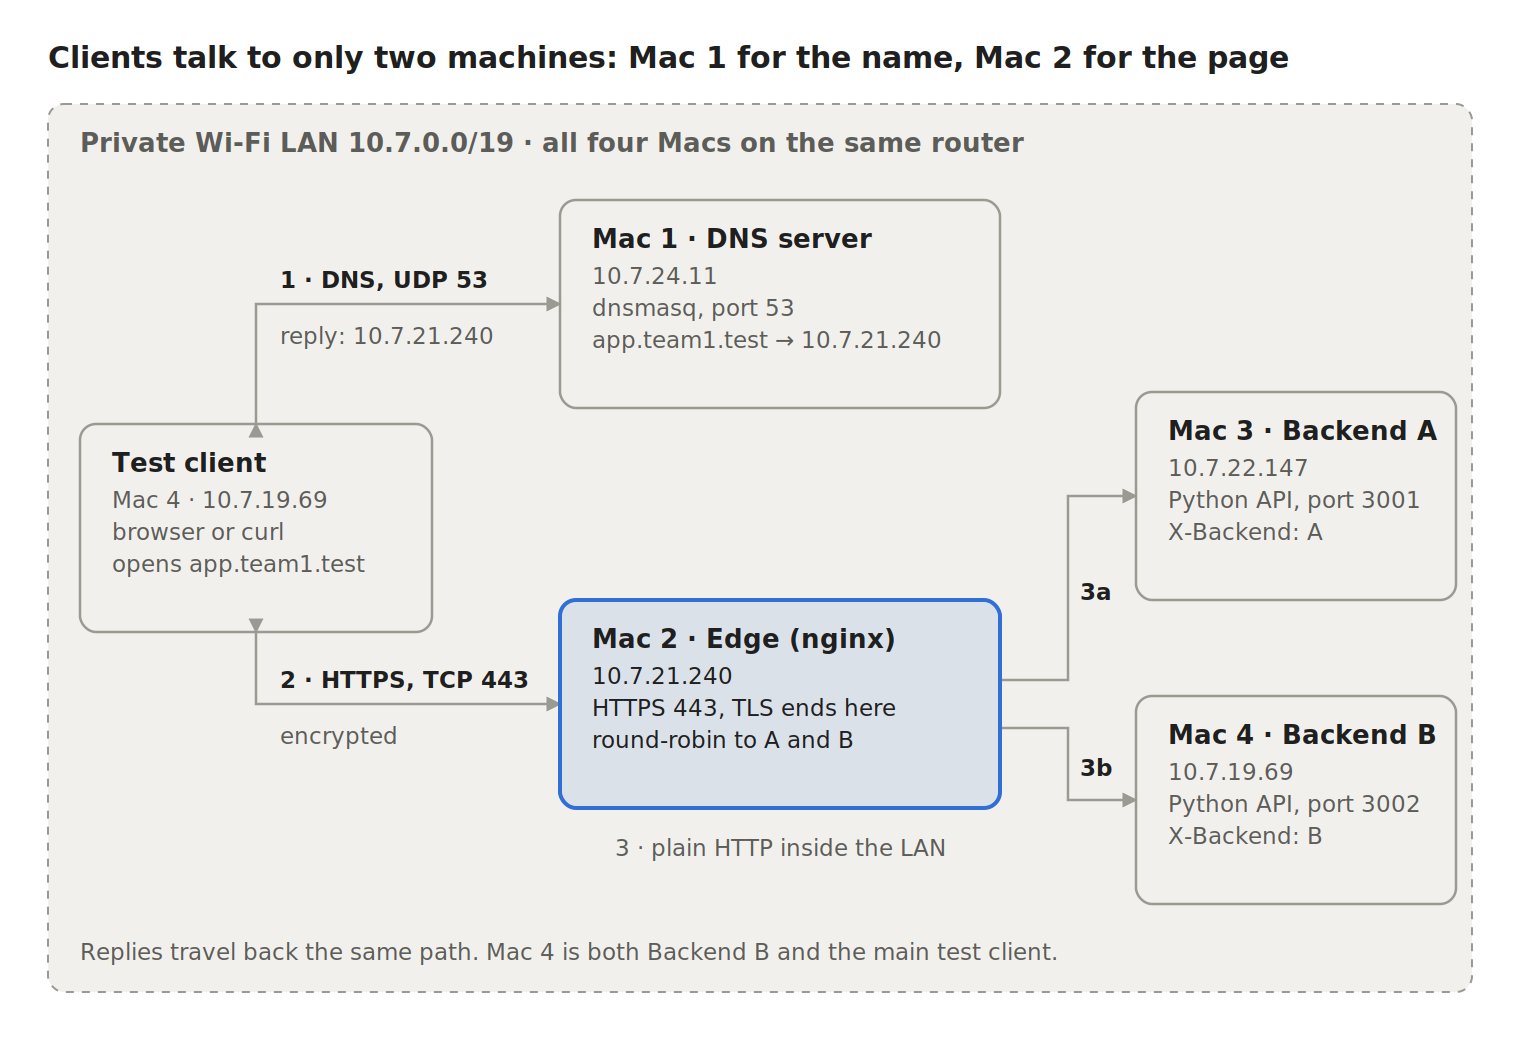
\includegraphics[width=\columnwidth]{phase1-topology.png}
\caption{Phase 1 topology and request path (addresses as recorded in
Phase 1).}\label{fig:p1}
\end{figure}

\subsection{Request path}
A client resolves \code{app.team1.test} through Mac 1 (UDP 53) and
receives Mac 2's address with a TTL of 30\,s. It opens TCP to Mac 2 port
443, completes a TLS handshake against a certificate signed by our own
root CA, and sends the HTTP request inside TLS (HTTP/2 by default). nginx
decrypts it and forwards plain HTTP to Backend A or B in round-robin
order; each backend marks its reply with \code{X-Backend}
(Fig.~\ref{fig:p1}). The client never learns a backend address.

\subsection{Phase 1 results}
Table~\ref{tab:p1} summarises the Phase 1 evidence stored in the
repository.

\begin{table}[t]
\caption{Phase 1 Results}\label{tab:p1}
\centering\footnotesize
\begin{tabular}{@{}p{1.6cm} p{6.1cm}@{}}
\toprule
Task & Observed result\\
\midrule
LAN & 0\% ping loss between every pair of Macs\\
DNS & Two clients resolve both names via Mac 1; TTL 30\,s\\
Backends & \code{/}, \code{/api/status}, \code{/api/info}; header \code{X-Backend}\\
Edge & Responses alternate A, B, A, B; HTTP/1.1 and HTTP/2 both served\\
TLS & Own root CA, SANs for both names, validation never skipped\\
Caching & \code{max-age=60} and a shared ETag; conditional request returns 304\\
Captures & DNS query/answer, SYN/SYN-ACK/ACK, TLS 1.2 handshake with
visible Certificate, TLS 1.3 with encrypted Certificate\\
Failures & Wrong resolver: name fails, ping works. Wrong record: TCP
refused. One backend down: all requests served by B. Both down: 502 from
the edge. Wrong port: TCP refused\\
\bottomrule
\end{tabular}
\end{table}

\section{Phase 2 Design}\label{sec:design}
Table~\ref{tab:changes} lists what Phase 2 adds; Fig.~\ref{fig:p2} shows
the resulting topology. No Phase 1 component was rebuilt.

\begin{table}[t]
\caption{What Changed from Phase 1}\label{tab:changes}
\centering\footnotesize
\begin{tabular}{@{}l p{3.1cm} p{2.9cm}@{}}
\toprule
Ext & Addition & Where\\
\midrule
A & Backup resolver, same records & dnsmasq on Mac 3; both clients list Mac 1, then Mac 3\\
B & Record change observed under a 30\,s TTL & Mac 1, Mac 3\\
C & Backend ports open to the edges only & \code{pf} anchor on Mac 3 and Mac 4\\
D & Passive health checks & nginx upstream on Mac 2\\
E & Standby edge and DNS cutover & nginx on Mac 3, own key\\
F & Layered diagnosis procedure & Client (Mac 4)\\
\bottomrule
\end{tabular}
\end{table}

\begin{figure*}[t]
\centering
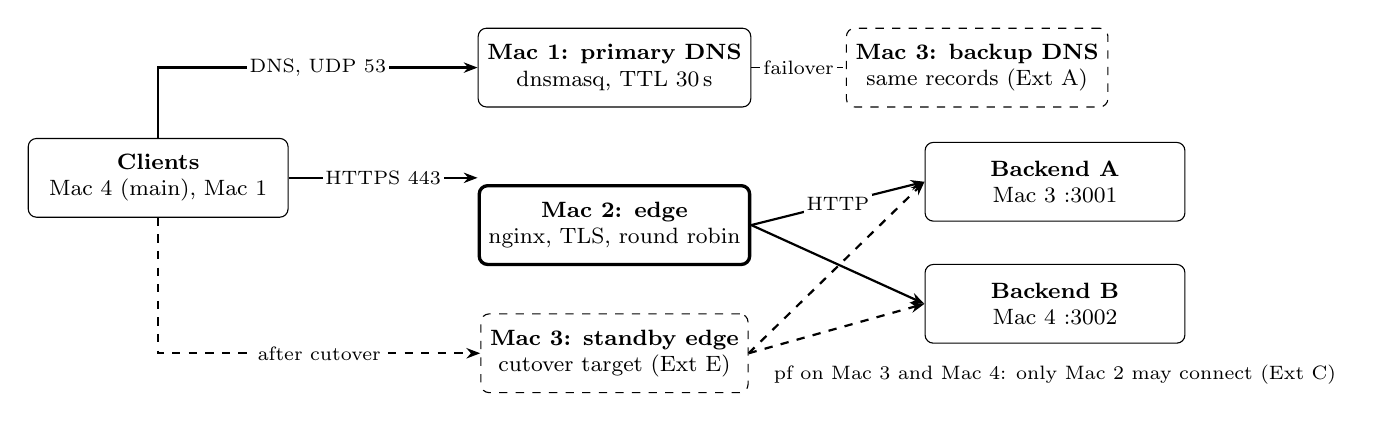
\begin{tikzpicture}[
  box/.style={draw, rounded corners=3pt, align=center, minimum width=3.3cm, minimum height=1cm, font=\footnotesize},
  dbox/.style={box, dashed},
  edge/.style={-{Stealth[length=5pt]}, thick},
  lab/.style={font=\scriptsize, fill=white, inner sep=1pt}]
\node[box] (client) {\textbf{Clients}\\Mac 4 (main), Mac 1};
\node[box, right=2.4cm of client, yshift=1.4cm] (dns1) {\textbf{Mac 1: primary DNS}\\dnsmasq, TTL 30\,s};
\node[dbox, right=1.2cm of dns1] (dns3) {\textbf{Mac 3: backup DNS}\\same records (Ext A)};
\node[box, right=2.4cm of client, yshift=-0.6cm, line width=1.2pt] (edge2) {\textbf{Mac 2: edge}\\nginx, TLS, round robin};
\node[dbox, below=0.6cm of edge2] (edge3) {\textbf{Mac 3: standby edge}\\cutover target (Ext E)};
\node[box, right=2.2cm of edge2, yshift=0.55cm] (ba) {\textbf{Backend A}\\Mac 3 :3001};
\node[box, right=2.2cm of edge2, yshift=-1.0cm] (bb) {\textbf{Backend B}\\Mac 4 :3002};
\node[font=\scriptsize, align=center, below=0.15cm of bb] (fw) {pf on Mac 3 and Mac 4: only Mac 2 may connect (Ext C)};
\draw[edge] (client) |- node[lab, pos=0.75] {DNS, UDP 53} (dns1);
\draw[dashed] (dns1) -- node[lab] {failover} (dns3);
\draw[edge] (client.east) -- node[lab] {HTTPS 443} (edge2.west |- client.east);
\draw[edge, dashed] (client.south) |- node[lab, pos=0.75] {after cutover} (edge3.west);
\draw[edge] (edge2.east) -- node[lab] {HTTP} (ba.west);
\draw[edge] (edge2.east) -- (bb.west);
\draw[edge, dashed] (edge3.east) -- (bb.west);
\draw[edge, dashed] (edge3.east) -- (ba.west);
\end{tikzpicture}
\caption{Phase 2 topology. Dashed elements are added in Phase 2; health
checks on the edge (Ext D) remove a failed backend from rotation.}\label{fig:p2}
\end{figure*}

\subsection{Ext A: backup DNS resolver}
Mac 3 runs a second dnsmasq instance with the same records, local zone and
TTL as Mac 1. Clients list Mac 1 first and Mac 3 second, so the backup is
consulted only when the primary does not answer.
\begin{lstlisting}
listen-address=127.0.0.1,10.7.10.192
local=/team1.test/
host-record=app.team1.test,10.7.31.128
host-record=api.team1.test,10.7.31.128
local-ttl=30
\end{lstlisting}

\subsection{Ext B: TTL and controlled record change}
Both resolvers serve the project records with a 30\,s TTL. A client
script (\code{watch-edge.sh}) prints, every 3\,s, the address returned by
the operating system resolver and the \code{X-Edge} header of the server
that answered. We change the record while it runs and compare it with
\code{dig}, which bypasses the OS cache.

\subsection{Ext C: service isolation}
Backends listen on all interfaces so that the edge can reach them, which
also lets any client bypass the edge. On Mac 3 and Mac 4 we load
\code{pf} rules into a separate anchor so that only the edge (Mac 2) may
open ports 3001 and 3002. \code{block return} rejects other clients
instead of silently dropping their packets, so they fail quickly rather
than timing out. The system file \code{/etc/pf.conf} is never edited; a
copy is kept for comparison and rollback is a single flush of the anchor.
The standby edge is not in the list, so the rules are rolled back before
the Ext E cutover.
\begin{lstlisting}
pass in quick proto tcp from 10.7.31.128 to any port { 3001, 3002 }
block return in quick proto tcp from any to any port { 3001, 3002 }
\end{lstlisting}

\subsection{Ext D: high-availability failover}
Open-source nginx performs passive health checks. With
\code{max_fails=1 fail_timeout=10s}, one failed connection removes a
backend from rotation for 10\,s, and \code{proxy_next_upstream} retries
the same request on the other backend, so the client sees no error.
\code{proxy_connect_timeout 2s} bounds the delay when a host is down
rather than refusing.

\subsection{Ext E: standby edge and DNS-based cutover}
Mac 3 runs a second nginx with the same backend pool and TLS settings. It
does not reuse Mac 2's private key: Mac 3 generates its own key and a
certificate signing request, and the team root CA on Mac 2 signs it.
Clients already trust that CA, so no client change is needed. The standby
adds \code{X-Edge: mac3-standby} (the primary sends \code{mac2}), so
every response shows which edge served it. Cutover is a single record
change from 10.7.31.128 to 10.7.10.192 on both resolvers.

\subsection{Ext F: diagnosis procedure}
For an unknown fault we test one layer at a time from the client and
stop at the first failure: \code{dig} (DNS), \code{ping} (IP),
\code{nc -vz} to port 443 (TCP), \code{openssl s_client} with the team CA
(TLS), and \code{curl -i} (HTTP and application). A 502 at the last step
moves the search behind the edge, to its error log and the backends.

\section{Experiments and Results}\label{sec:results}
All tests ran on 24 November 2026. The runbook (\code{phase2/README.md})
lists every command; screenshots and transcripts are in
\code{evidence/Phase-2}.

\subsection{Ext A}
The backup resolver on Mac 3 answered \code{app.team1.test} and
\code{api.team1.test} with 10.7.31.128 and TTL 30 in 3\,ms, and forwarded
an external name upstream. Mac 4 queried it directly and received the
same answer. With both resolvers configured on Mac 3 (10.7.18.129 first),
a normal lookup was answered by the primary (\code{SERVER: 10.7.18.129},
24\,ms): the backup stays idle while the primary is healthy.
\pending{primary on Mac 1 stopped; client lookup answered by
10.7.10.192; HTTPS result; backup log line; primary restored}.

\subsection{Ext B}
A lookup from Mac 1 returned \code{app.team1.test. 30 IN A 10.7.31.128}.
\pending{record change; time until the client's OS resolver switched
(expected at most 30\,s); \code{dig} vs.\ OS cache at the same moment;
manual flush}.

\subsection{Ext C}
Table~\ref{tab:iso} lists the results; Fig.~\ref{fig:iso} shows the
client side. Blocked connections failed with curl error 7,
\emph{Couldn't connect to server}, after about 1\,s, well inside the 5\,s
limit, so they were rejected rather than left to time out. Requests
through the edge kept succeeding, and Mac 2 could still reach Backend A
directly. Rollback flushed the anchor and disabled pf on both backends,
and \code{diff} showed \code{/etc/pf.conf} unchanged.

\begin{table}[t]
\caption{Ext C: Access to the Backends}\label{tab:iso}
\centering\footnotesize
\begin{tabular}{@{}p{2.5cm} p{2.3cm} p{2.6cm}@{}}
\toprule
Request & Before rules & With rules\\
\midrule
Mac 1 $\to$ A (direct) & 200, backend A & refused after 1018\,ms\\
Mac 1 $\to$ B (direct) & not captured & refused after 1008\,ms\\
Mac 1 $\to$ edge (HTTPS) & 200, backend B & 200, backend A\\
Mac 2 $\to$ A (direct) & not captured & 200, backend A\\
\bottomrule
\end{tabular}
\end{table}

\begin{figure}[t]
\centering
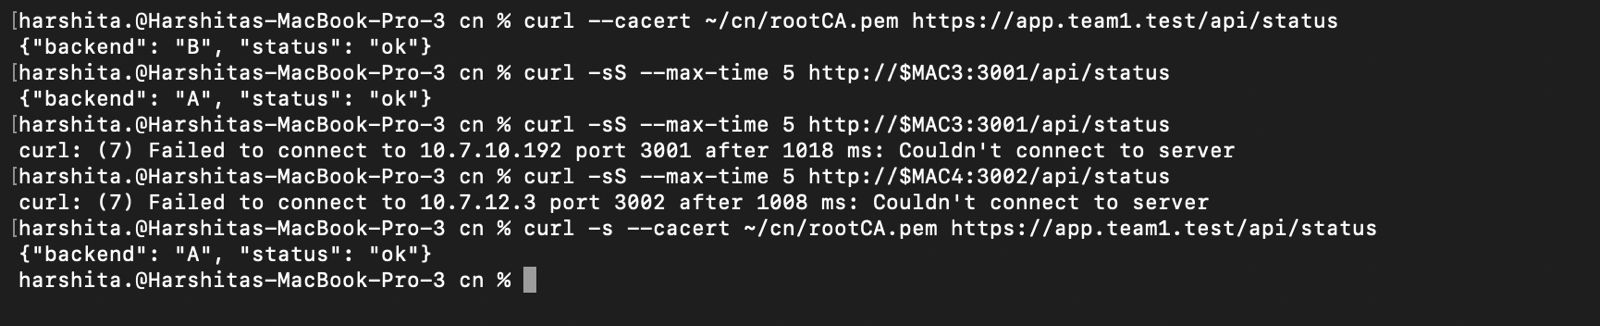
\includegraphics[width=\columnwidth]{../../evidence/Phase-2/C-Isolation/blocked-mac1.jpg}
\caption{Ext C on Mac 1: direct access to ports 3001 and 3002 refused
once the rules are loaded; the same request through the edge succeeds.}\label{fig:iso}
\end{figure}

\subsection{Ext D}
A loop on Mac 4 printed the backend of each response. A and B alternated;
after Backend A was stopped, every printed response came from B. At
18:26:14 nginx logged \emph{connect() failed (61: Connection refused)
while connecting to upstream} for \code{10.7.10.192:3001}, on a request
from 10.7.12.3, and served that request from B:


\begin{lstlisting}
2026/11/24 18:26:14 [error] 34468#0: *117 kevent() reported that
connect() failed (61: Connection refused) while connecting to upstream,
client: 10.7.12.3, server: app.team1.test,
request: "GET /api/status HTTP/2.0",
upstream: "http://10.7.10.192:3001/api/status"
\end{lstlisting}
A second, timestamped run from Mac 3 sent requests straight to Mac 2.
Eight baseline requests alternated between B and A. Backend A was killed
at 18:59:05; the next ten requests (18:59:06--18:59:14) all returned 200
from B. Backend A was restarted at 18:59:15 and served its first request
again at 18:59:21, 6\,s later, within the 10\,s \code{fail_timeout} after
which nginx retries a failed upstream; from then on A and B alternated.

\subsection{Ext E}
Before the cutover, responses on Mac 1 carry \code{x-edge: mac2} with
\code{HTTP/2 200}. \pending{standby ready with \code{x-edge: mac3-standby};
cached client kept reaching Mac 2 for N\,s after the change; fresh client
reached Mac 3 at once; rollback}.

\subsection{Ext F}
\pending{fault injected by faculty; layer at which the first check
failed; root cause; fix; time to diagnose}.

\section{Troubleshooting Findings}\label{sec:trouble}
Three problems arose while setting up Phase 2. Each was located with the
same layered method as Ext F.

\subsubsection{Address changes}
Between the phases the lab DHCP server gave all four Macs new addresses,
and Mac 4 reported a second new address during setup. Every component
that stores an address had to change: the DNS records, the nginx upstream
pool and the verification scripts. The TLS certificates did not, because
their subject alternative names are host names. This is the practical
argument for naming services instead of addresses, and for DHCP
reservations on servers.

\subsubsection{Port 53 already in use}
Starting the backup resolver on Mac 3 failed with \emph{failed to create
listening socket for 10.7.10.192: Address already in use}. A dnsmasq
started earlier as a Homebrew service still held UDP 53. Stopping that
service freed the socket; a socket can have only one owner per address and
port.

\subsubsection{Host firewall dropping DNS}
With the resolver running, \code{dig @127.0.0.1} answered but
\code{dig @10.7.10.192} timed out. The service was healthy, so the fault
lay between the network and the application. The macOS application
firewall listed dnsmasq as \emph{Block incoming connections}. Allowing it
fixed the query. The symptom, a timeout and not a refusal, pointed to a
silent drop rather than a closed port.

\section{Discussion}\label{sec:discussion}

\subsection{DNS failure versus application failure}
When the resolver fails, the name cannot be turned into an address
although every server is healthy; the client reports that the host cannot
be resolved. When the application fails, resolution and the TLS handshake
still succeed and the edge returns 502. The first visible error therefore
identifies the layer.

\subsection{Cost of a short TTL}
A 30\,s TTL bounds how long clients keep an old answer, which makes
cutover fast, at the price of more queries to the resolver. Production
migrations lower the TTL in advance, change the record, keep the old
endpoint serving for at least one old TTL, and raise the TTL again.

\subsection{Remaining single point of failure}
Backends and resolvers are now redundant. The active edge is not: if Mac 2
fails, clients that cached its address keep failing for up to one TTL,
and someone must change the record. Two edges behind one floating address
(VRRP with keepalived) or a health-checked DNS service would remove this.
Table~\ref{tab:cloud} maps our components to managed cloud equivalents.

\begin{table}[t]
\caption{Phase 2 Components and Cloud Equivalents}\label{tab:cloud}
\centering\footnotesize
\begin{tabular}{@{}p{3.3cm} p{4.4cm}@{}}
\toprule
This project & Cloud equivalent\\
\midrule
Primary + backup dnsmasq & Multiple authoritative name servers (Route 53)\\
Record change under TTL & Weighted / failover routing records\\
\code{pf} edges-only rule & Security group allowing only the load balancer\\
nginx passive health check & Target health checks (ALB)\\
Standby edge + DNS cutover & Multi-zone load balancer with DNS failover\\
\bottomrule
\end{tabular}
\end{table}

\section{Learning Summary}
\textbf{Ext A.} Redundancy in DNS lives in the client: a second server
helps only because the client's resolver list names it and the client
tries it when the first fails.

\textbf{Ext B.} A record change is not a switch but a gradual drain; how
fast it reaches clients is set by the TTL chosen before the change.

\textbf{Ext C.} Binding to all interfaces makes a service reachable, and
reachability must then be narrowed on purpose. A host firewall does this
without touching the application.

\textbf{Ext D.} A load balancer that retries on another upstream turns a
backend failure into extra latency rather than an error, as long as one
healthy backend remains.

\textbf{Ext E.} Moving an edge needs the same trust (a certificate from
the same CA), the same pool, and a DNS change; existing clients follow
only after their cached answer expires.

\textbf{Ext F.} Checking layers in order, and noting whether a failure is
a refusal or a timeout, finds the faulty layer faster than guessing.

\section{Conclusion}
Phase 2 adds a backup resolver, a firewall on the backends, health-checked
load balancing and a standby edge to the Phase 1 network.
\pending{summary of which failures the system now survives, from
Section~\ref{sec:results}}. The remaining single point of failure is the
active edge, and the fix is a floating address or health-checked DNS.

\begin{thebibliography}{10}
\bibitem{rfc1034} P. Mockapetris, ``Domain names---concepts and facilities,'' RFC 1034, 1987.
\bibitem{rfc1035} P. Mockapetris, ``Domain names---implementation and specification,'' RFC 1035, 1987.
\bibitem{rfc2181} R. Elz and R. Bush, ``Clarifications to the DNS specification,'' RFC 2181, 1997.
\bibitem{rfc6761} S. Cheshire and M. Krochmal, ``Special-use domain names,'' RFC 6761, 2013.
\bibitem{rfc9293} W. Eddy, Ed., ``Transmission Control Protocol (TCP),'' RFC 9293, 2022.
\bibitem{rfc5246} T. Dierks and E. Rescorla, ``The Transport Layer Security (TLS) protocol version 1.2,'' RFC 5246, 2008.
\bibitem{rfc8446} E. Rescorla, ``The Transport Layer Security (TLS) protocol version 1.3,'' RFC 8446, 2018.
\bibitem{rfc9110} R. Fielding, M. Nottingham and J. Reschke, Eds., ``HTTP semantics,'' RFC 9110, 2022.
\bibitem{rfc9111} R. Fielding, M. Nottingham and J. Reschke, Eds., ``HTTP caching,'' RFC 9111, 2022.
\bibitem{rfc9113} M. Thomson and C. Benfield, Eds., ``HTTP/2,'' RFC 9113, 2022.
\bibitem{rfc5798} S. Nadas, Ed., ``Virtual Router Redundancy Protocol (VRRP) version 3,'' RFC 5798, 2010.
\bibitem{nginx} nginx documentation, ``Module ngx\_http\_upstream\_module.'' [Online]. Available: \url{https://nginx.org/en/docs/http/ngx_http_upstream_module.html}
\bibitem{dnsmasq} S. Kelley, ``dnsmasq(8) manual page.'' [Online]. Available: \url{https://thekelleys.org.uk/dnsmasq/docs/dnsmasq-man.html}
\bibitem{pf} OpenBSD, ``pf.conf(5) manual page.'' [Online]. Available: \url{https://man.openbsd.org/pf.conf}
\end{thebibliography}

\end{document}
